\section{Searching for the signal}
\begin{marginfigure}
	\centering
	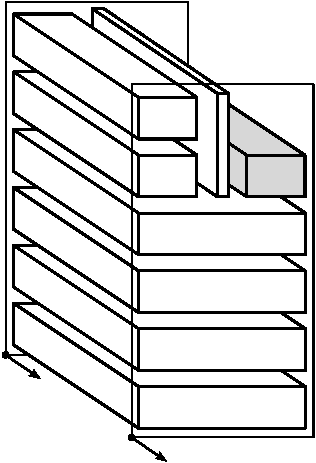
\includegraphics[scale=0.5]{ch3/img/PA_map_exploration.pdf}
\end{marginfigure}
In this section we derive a very simple method to cover the avalanche front to search for a signal beacon. The algorithm presented is incredibly simple and derives from what is actually done by a rescuer on the avalanche front. We try to cover the area of the avalanche with straight equi--spaced lines generated from a series of points.
\begin{figure*}[p]
\caption{Exploration algorithm} \label{fig:exploration} \centering
\begin{tikzpicture}[auto,node distance=0.5cm and 1cm, >=latex', minimum width=3cm, minimum height=1cm, text width=4cm, align=center]

	%\draw (0,0) ellipse (2cm and 1cm) node (start) {Start};
	%\draw

	\node [ellipse, draw, minimum width=2cm, text width=2cm, fill=gray!40] (start) {Start};
	\node [trapezium, draw, trapezium left angle=70,trapezium right angle=-70, below=of start] (inserimento) {Receiving starting point $\mathbf{p}_0$, ending point $\mathbf{p}_n$, plane direction};
	\node [rectangle, draw, below=of inserimento] (generazione_punti) {Generation of points vector $\mathbf{P} = [\mathbf{p}_0,\dots,\mathbf{p}_n]$, set confidence distance $\Delta$};
	\node [rectangle, draw, below=of generazione_punti] (abilita_ricerca) {Start searching sensors, start radar detection routines $\Lambda(\mathbf{s}) \overset{?}{<>} \eta$ };
	\node [rectangle, draw, below=of abilita_ricerca] (goto_start) {$i \leftarrow 0$};
	\node [rectangle, draw, below=of goto_start, text width=2cm] (select_point) {Go To $\textbf{p}_i$};
	\node [trapezium, draw, trapezium left angle=70, trapezium right angle=-70, below=of select_point,text width=1.2cm] (read_position) {Get $\mathbf{x}$};
	\node [diamond, draw, aspect=2, text width=2.3cm, below=of read_position] (distanza) {$\left| \mathbf{p}_i - \mathbf{x} \right| < \Delta$ ?};
	\node [diamond, draw, aspect=2, text width=2cm, below=of distanza] (lastpoint) {$i = n$ ?};
	\node [ellipse, draw, minimum width=2cm, text width=2cm, below=of lastpoint,fill=gray!40] (stop) {Stop};

	\node [rectangle,draw,left=of lastpoint, text width=1.5cm] (addone) { $i \leftarrow i+1$ };
	\coordinate [at=(select_point.north), shift=(0:22mm)] (braces_a);
	\coordinate [at=(distanza.south), shift=(0:22mm)] (braces_b);
	\draw [decorate,decoration={brace,amplitude=12pt}] (braces_a) -- (braces_b) {};

	\node [diamond, draw, aspect=2, text width=2cm, at=(read_position.north east), shift=(0:50mm)] (detection) {$\Lambda(\mathbf{s}) > \eta$?};
	\node [rectangle, draw,fill=gray!40, text width=2.5cm, below=of detection] (search) {Search \mbox{H--field} source};

	\coordinate [at=(detection.north), shift=(90:5mm)] (extraA);
	\coordinate [at=(search.south), shift=(270:5mm)] (extraB);
	\coordinate [at=(detection.west), shift=(180:5mm)] (extraC);
	\coordinate [at=(distanza.west), shift=(180:10mm)] (intraB);

	\draw [->] (start) -- (inserimento);
	\draw [->] (inserimento) -- (generazione_punti);
	\draw [->] (generazione_punti) -- (abilita_ricerca);
	\draw [->] (abilita_ricerca) -- (goto_start);
	\draw [->] (goto_start) -- coordinate[pos=0.5](intraA) (select_point);
	\draw [->] (select_point) -- (read_position);
	\draw [->] (read_position) -- (distanza);
	\draw [->] (distanza) -- node[shift=(0:-17mm)]{\scriptsize{true}} (lastpoint);
	\draw [->] (lastpoint) -- node[shift=(0:-17mm)]{\scriptsize{true}} (stop);
	\draw [->] (detection) -- node[shift=(0:-17mm)]{\scriptsize{true}} (search);
	\draw [->] (lastpoint) -- node[shift=(45:3mm)]{\scriptsize{false}} (addone);

	\draw [->,dashed] (extraA) -- (detection);
	\draw [->,dashed] (search) -- (extraB);
	\draw [->,dashed] (detection) -- node[shift=(45:3mm)]{\scriptsize{false}} (extraC);

	\draw [->] (addone) |- (intraA);
	\draw (distanza) -- node[shift=(45:3mm)]{\scriptsize{false}} (intraB) |- (intraA);

\end{tikzpicture}
\end{figure*}

When turned on, the drone require insertion of two GPS coordinates, or  and a direction from the rescuer. Those two coordinates represent starting point and ending point for the first level of search. Those two points defines a rectangle, the direction represent the orientation of the rectangle. Those data could be inserted from a media device such as tablet or smarthphone.

Once the search area is defined, it is divided into a regular grid, identified by points in the center of each square of the grid. Due to the fact that such input derives from an external device that has computational power, we could use this external device to perform such calculation.

Once the points array is defined, drone simply uses the lower levels of the map to reach each point in sequence. In some cases may be impossible to reach the specific point, due to causes like obstacle or uncertainty due to the motion. To avoid this problem, for each point, is associated a confidence distance, that defines a sphere in which the drone should fly before going to the next point. When last point is reached mission is over. A flowchart of algorithm is presented in figure \ref{fig:exploration}.

\TODO{Immagine esplicativa}

\section{Source searching algorithm}

Some new papers in searching suggested the use of a modified version of the \emph{SLAM} problem to identify position of the source and direction of the dipole. Even if some promising results are exposed in cited papers \citep{pinies2006fast,pinies2006localization}, we were not able to reproduce such results with our system in simulations; because of that, we decided to drop this approach to use one that fit better the perception--action paradigm.

The proposed algorithm uses a two component algorithm.

\subsection{Exploration step}
\begin{marginfigure}
	\centering
	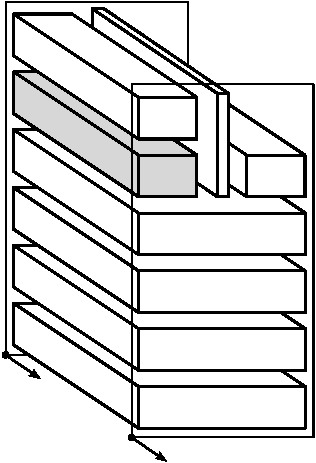
\includegraphics[scale=0.5]{ch3/img/PA_map_direction.pdf}
\end{marginfigure}
The first step is simply an adaptive filter, stolen from the evaluation of Round--Trip--Time in TCP networking, that tries to identify a direction in which the signal is maximized, given an adapted previous knowledge. The algorithm takes into consideration the presence of fluctuations due to noise and interference and changes orientation only when the change in signal is obvious. Scaling parameter regulate the velocity that will move the drone.

An adaptive filter for a variable $x$ is defined as:
\[
x_k = \alpha x_{k-1} + (1-\alpha) \hat{x}_k \qquad 0 \leq \alpha \leq 1
\]

The first part is a mean sampler, that helps us to partially eliminate the white Gaussian noise:
\begin{equation}
	\hat{\hfield}_g = \dfrac{1}{N} \rotmat \sum\limits_{i=0}^{N} \hfield_{b,i}
\end{equation}
Starting from the vector of received signal $\hfield$, the value measured is a vector in hexa--copter body reference frame, and should be reported in ground reference frame, using the state of the drone. From the projection of the H--field some information are extracted, like \textbf{intensity} and \textbf{direction on} $(\vrx\times\vry)$ \textbf{plane}:
\begin{equation}
\begin{array}{rcl}
	\ccos{\alpha} & = & \ccos{\arctan_2(H_y,H_x)} \\
	\ssin{\alpha} & = & \ssin{\arctan_2(H_y,H_x)} \\
	\abs{\hfield} & = & \sqrt{H_x+H_y+H_z}
\end{array}
\end{equation}
The next step is a filtering to eliminates some of the residual noise, with a second order filter. We exploit the discontinuity problem of the ${\arctan_2(\cdot)}$ function using trigonometric functions. From the input values:
\begin{itemize}
\item the value of the measured field is used to steer the system in direction of the source, to avoid symmetric problem of the received field
\item the adapted H--field measurement defines the speed, throug a function ${v(\cdot)}$
\item the direction of speed is defined using adapted angle
\end{itemize}
The effect of this routine is only to explore the environment in a direction the maximizes the received signal.

\begin{algorithm}
\caption{Searching and explore}
\KwData{$|\hfield|_{k-1},\,\psi_{k-1},\,\mathbf{v}_{k-1},\,w_1,\,w_2,\,\Delta,\,\delta$}
\tcc{Steer in direction of greater intensity}
\If{$\braces{\dfrac{|\hfield|_k}{|\hfield|_{k-1}} - 1 } \leq \Delta$}{
	$\psi_k = (1-w_1)\psi_{k-1} + w_1 \delta$\;
}
\ElseIf{$\braces{\dfrac{|\hfield|_k}{|\hfield|_{k-1}} - 1 } \geq \Delta$}{
	$\psi_k = (1-w_1)\psi_{k-1} - w_1 \delta$\;
}

\tcc{Set speed magnitude}
$|\mathbf{v}_{k}| = (1-w_2) |\mathbf{v}_{k-1}| + w_2 v(|\hfield_k|)$\;

\tcc{Steer in direction of flux lines}
$\ccos{\psi}_k = (1-w_1) \ccos{\theta} + w_1 \ccos{\psi}_{k-1} $\;
$\ssin{\psi}_k = (1-w_1) \ssin{\theta} + w_1 \ssin{\psi}_{k-1} $\;

\tcc{Defines speed}
\renewcommand{\arraystretch}{1}
$\mathbf{v}_k = \vettore{
	|\mathbf{v}_k| \ccos{\psi}_k \\
	|\mathbf{v}_k| \ssin{\psi}_k \\
	0
}$\;
\renewcommand{\arraystretch}{1.75}
\Return{$\mathbf{v}_k$}
\end{algorithm}

\subsection{Emulation step}
\begin{marginfigure}
	\centering
	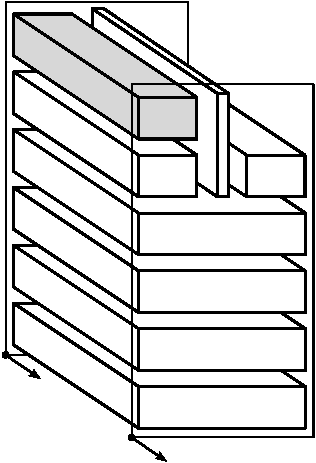
\includegraphics[scale=0.5]{ch3/img/PA_map_emulation.pdf}
\end{marginfigure}

\myparagraph{Optimization}
In parallel with the previous searching method, an emulation of the real field is implemented. The emulation tries to understand the position of the source as a solution of an optimization problem, using previous solution as a guess that is adapted through time. The optimization problem is:
\begin{equation}
\begin{array}{ll}
\underset{\mathbf{p}_T}{\mathrm{arg~min}} & \boldsymbol{\delta} \\
\mathrm{subject~to} & 	\left\{ \begin{array}{l}
							\boldsymbol{\delta} = \braces{\hfield(\hexastate,\mathbf{p}_T, \mathbf{m}) - \hat{\hfield}}^2 \\
							\braces{\hexastate - \mathbf{p}_T}^2  \leq  {\radiodist_{\mathrm{max}}}
						\end{array} \right. \\ 
\end{array}
\end{equation}
The optimization problem is solved numerically, guessing as initial point the solution at the previous step. The unilateral constraint is transformed in a barrier function.

The solution of the optimization routine is saved in a persistent memory, as a vector:
\[ \mathbf{P} = [ \mathbf{p}_{T,k} \,:\, k=1..N ] \]

\myparagraph{Estimation}
At this point, with could notice a lot of fluctuation in the solution, due to the noise in measurement, that is why we decided to treat the solution as a stochastic process. The solution are parsed in a \emph{parzen window estimator}, a non--parametric estimator, that consider a kernel function $\kernel$ with volume $V(h)$:
\begin{itemize}
\item $h$ identifies a kernel geometric characteristic
\item the kernel is normal: 
\[ \int\limits_{\mathbb{R}^n} \dfrac{\kernel}{V(h)}d\mathbf{p} = 1 \]
\item $\gamma(\cdot)$ has maximum in the origin
\item $\gamma(\cdot)$ is continuous
\item $\gamma(\pmb{\mu}\leftarrow\infty)\leftarrow 0$
\end{itemize}
the approximation of the distribution of the solution of the optimization step is in the form:
\begin{equation}
\hat{p}(\mathbf{p}) = \dfrac{1}{N}\sum\limits_{k=1}^{N} \dfrac{\gamma(\mathbf{p}-\mathbf{p}_k,h)}{V(h)}
\end{equation}
We have chosen as kernel a Gaussian function: 
\[ \int\limits_{-\infty}^{\infty} \dfrac{1}{\sqrt{2\pi} h} e^{-\dfrac{z^2}{2 h^2}} dz = 1 \]
Such an estimator has the following drawbacks:
\begin{itemize}
\item with the exact knowledge of the distribution that we are trying to estimate, the expectation of the estimation shows us that such an estimation is a blurred version of the real one: \[{E\{\hat{p}(\mathbf{p})\} = p(\mathbf{p}) * \dfrac{1}{h} \gamma(\mathbf{p},h)}\]
\item the estimation may suffer bias problem for samples $N<\infty$, that means \[{E\{\hat{p}(\mathbf{p})\}=E\{{p}(\mathbf{p})\} + \Delta}\]
\end{itemize}

The final concept of the estimator is to identify the position inside a certain circle of confidence. When the drone is in such a confidence area, it release the dart to signal the position to the rescue.